\documentclass[journal]{IEEEtran}
\usepackage[usenames]{color}
\usepackage{epsfig}
\usepackage{graphics}
\usepackage{caption}
\usepackage{amsmath}
\usepackage{amssymb}
\usepackage{multirow}
\usepackage{cite}
\usepackage{array}
\usepackage{url}
\usepackage{lineno}
\usepackage{graphicx}
\usepackage{setspace}
\usepackage{tikz}
\usepackage{mathtools}
\usepackage{xcolor}
\usepackage{bm}
\usepackage{bbm}
\usepackage{booktabs}
\usepackage{mdframed}
\usepackage[letterpaper]{geometry}
\geometry{verbose,tmargin=0.55in,bmargin=1.0in,lmargin=0.65in,rmargin=0.65in}
\setlength{\headheight}{48pt}
\setlength{\headsep}{14pt}

% 中文支持
\usepackage{xeCJK}
\setCJKmainfont{SimSun}
\setCJKsansfont{Microsoft YaHei}
\setCJKmonofont{Microsoft YaHei}

\renewcommand{\abstractname}{\textcolor{violet}{\textbf{ABSTRACT / 摘要}}}
\newcommand{\flogo}{
\includegraphics[height=40pt]{LOGO1.png}}

\pagenumbering{gobble}

\usepackage{fancyhdr}
\pagestyle{fancy}
\fancyhf{}
\lhead{\flogo}
\rhead{
\includegraphics[height=40pt]{LOGO2.png} \thepage}
\pagestyle{fancyplain}

\makeatletter
\ifCLASSOPTIONjournal
\def\abstract{\@IEEEtweakunitybaselinestretch{1.15}
	\@IEEEabskeysecsize\noindent\abstractname---\relax
	\fi\@IEEEgobbleleadPARNLSP}
\makeatother

\newcommand{\citet}[1]{\cite{#1}}

% 灰色聊天日志框
\newmdenv[
  backgroundcolor=gray!10,
  linecolor=gray!40,
  linewidth=0.5pt,
  roundcorner=4pt,
  innertopmargin=6pt,
  innerbottommargin=6pt,
  innerleftmargin=8pt,
  innerrightmargin=8pt,
  font=\small\ttfamily
]{chatbox}

\begin{document}

\title{\vspace*{0.5cm}\textcolor{violet}{基于多智能体博弈的"薛定谔的鸽子"演化模型：\\
当代社交承诺中"下次一定"的次贷危机推演}
\vspace*{0.3cm}
}

\author{\textbf{鸽子博弈研究组$^{1}$，S.H.I.T. 期刊编辑部$^{2}$}\\
\vspace*{0.1cm}
中国北京 薛定谔大学 社会信用研究所 \\
\vspace*{0.2cm}
\small
$^{1}$ 薛定谔大学鸽子行为学系，朝阳区，北京 \\
$^{2}$ S.H.I.T. 整活研究中心，朝阳区，北京 \\
\vspace*{0.1cm}
通讯作者：鸽王（e-mail: never-show-up@shitspace.xyz）\\
\vspace*{0.1cm}
本研究由"下次一定"国家自然科学基金资助（项目编号：NEXT-TIME-114514）\\
本文包含完整52周模拟日志及开源框架源码 \\
\normalsize
}

\twocolumn[
\begin{@twocolumnfalse}
\let\newpage\relax\maketitle\thispagestyle{fancy}
\begin{abstract}
\textbf{目的：}本研究旨在揭示当代社交互动中"下次一定"这一语言承诺行为的系统性泡沫特征与次贷危机演化机制。
\textbf{方法：}基于多智能体推演框架，构建了包含五种典型社交人格的群聊环境（对照组），并设计了去除理性审计角色的消融实验（实验组）。两平行宇宙分别进行为期52周的模拟实验，引入5次外部冲击事件，每周记录群聊交互、社交债务演进及泡沫指数变化。
\textbf{结果：}对照组（含记账狂）债务总额从0元飙升至1,372元，泡沫破裂指数（SBBI）达到97.6（深红预警），累计兑现率仅59.2\%，信用均值从800崩溃至459。实验组（鱼系青年替代记账狂）债务总额仅501元，泡沫指数50.8（橙色预警），兑现率34.0\%，信用均值537，均优于对照组。异质性分析表明，降雨量每增加10mm，违约率上升约7.3\%（$p<0.05$）；MBTI中P型人格的平均承诺折扣率比J型高43.6\%。
\textbf{结论：}提出并验证了"透明度悖论"假说——系统中存在绝对理性的审计者时，因其高效率记录和追索行为加速了承诺-兑现的剪刀差膨胀，导致社交信用体系的更快崩溃。完整推演框架已开源至GitHub：\url{https://github.com/zhouder/Pigeon-Agent-Simulation}。
\\
\noindent
\textcolor{violet}{\textbf{INDEX TERMS / 关键词}} 下次一定，社交泡沫，薛定谔的鸽子，多智能体推演，庞氏结构，情感次贷，消融实验，透明度悖论，随机微分方程，异质性分析。\\
\\
\textcolor{violet}{\textbf{IMPACT STATEMENT / 影响声明}} 本文首次通过可控消融实验验证了"下次一定"作为一种社交信用衍生品的系统性脆弱性，并发现了审计者存在反而加速系统崩溃的反直觉现象。
\vspace{0.3cm}
\end{abstract}
\end{@twocolumnfalse}
]

\IEEEpeerreviewmaketitle

% =========================================================================
\section{INTRODUCTION / 引言}
% =========================================================================

\subsection{研究背景与动机}

"下次一定"——这一看似无害的社交用语，在当代青年的日常互动中已成为最具破坏力的修辞武器之一。从饭局邀约到还书承诺，从"改天喝咖啡"到"有空聚一下"，"下次一定"的使用频率已远超其兑现频率，形成了社会学意义上罕见的"承诺-兑现"剪刀差现象\citet{pigeon_linguistics}。

本研究将其命名为\textbf{"薛定谔的鸽子"}现象：当一个人说出"下次一定"时，在观测行为发生之前，该承诺同时处于"会兑现"和"不会兑现"的叠加态；然而一旦时间到达约定的观测点，波函数必然坍缩为"鸽子态"。这一量子社会学隐喻精确刻画了当代社交承诺的核心矛盾——承诺的真实状态只有在约定的兑现时刻才被决定，而系统的初始条件（社交信用积累、历史违约记录、当前借口质量）决定了坍缩的方向\citet{schrodinger_vs_pigeon}。

本质上，"下次一定"构成了一个\textbf{无抵押、无担保、无交割期限}的"三元缺失"社交信用衍生品\citet{ponzi_social}。每一次"下次一定"的发行，即是在社交关系账本上进行了一次无准备金信用扩张。当这种信用扩张的速度持续超越兑付速度时，一个微观层面的庞氏结构便在社会关系网络中悄然形成。

\subsection{历史溯源：从农业社会到信息时代的承诺演化}

理解"下次一定"现象不能脱离其历史背景。纵观人类社交承诺的演化史，我们可以清晰地辨识出三个阶段。

\textbf{农业社会的高兑现率时代。}在自给自足的小农经济中，社交承诺的违约成本极高——失信不仅意味着个人声誉的损失，更可能导致在缺乏正式契约保护的熟人社会中失去生存资源。费孝通先生所说的"差序格局"\citet{guanxi}本质上构成了一个高密度、低延迟的信用监督网络。在这种社会结构中，"下次一定"如果说出，兑现率可能超过85\%——因为不兑现的代价是"在整个村子失去信用"。承诺的兑现与社会物理距离成反比，与监督密度成正比。

\textbf{福特制工业时代的定时社交。}工业革命带来了标准化的时间规训——工厂的精确作息、工作日的固定节奏、下班后的有限社交窗口，社交互动的时间成本被压缩到可预测的时空框架中。在这种"福特制社交"模式下，承诺的兑现具有高度的可预期性：周五晚上就是社交时间，没有"下次"的模糊空间。社交债务的违约率维持在较低水平（估计约15-20\%），因为违约者需要面对面地向同事解释其缺席的合理性。

\textbf{信息时代的异步通讯革命。}互联网的诞生，尤其是移动即时通讯工具的普及，从根本上重构了社交承诺的时间结构。异步通讯（Asynchronous Communication）赋予了个体前所未有的"推延自由度"：发出承诺不需要即时兑现，作出约定不需要确定时间。微信等平台的"已读不回"功能更是创造了\textbf{沉默违约（Default by Silence）}这一新型失信模式——答应的那一刻是真的想赴约，但到了那天是真的不想出门。二者的矛盾在量子叠加态中获得统一。

当前中国互联网用户的"下次一定"日均使用频次约为2.7次（本实验室在2024年冬至2025年秋开展的大规模语料采集数据），远超其平均社交活动频次（约0.3次/周），形成了约63倍的\textbf{承诺-活动剪刀差}。这一量级已接近学术界公认的庞氏结构预警阈值。

\subsection{哲学与伦理学思辨}

从康德伦理学的视角审视，"下次一定"构成了一个极具张力的道德悖论。康德的\textbf{绝对命令}（Categorical Imperative）要求：一条道德准则必须可以普遍化而不产生矛盾。若将"下次一定但不兑现"作为普世准则推广——即每个人都期待别人的承诺但不兑现自己的承诺——这种普遍化将摧毁承诺体系本身，从而产生逻辑矛盾。因此，按照康德的伦理框架，"下次一定"行为在道德上是不可允许的。

然而，当代青年的社交实践却对这一古典伦理框架提出了严峻挑战。我们将其命名为\textbf{"碎片化功利主义"（Fragmented Utilitarianism）}：在微观层面上，每一个"下次一定"的决策都是个体在特定时间约束下的最优功利选择——呆在家里不出门的边际效用（看剧+吃零食+不洗头）显著高于赴约的边际效用（交通成本+社交精力消耗+必须洗头）。个体在面对"出门还是鸽掉"这一二元选择时，经过短暂的贝叶斯推理，通常得出"鸽掉利益最大化"的结论。

进一步地，从后现代主体性理论出发，"不想出门"可以被重新阐释为\textbf{主体性对现代时间规训的一种微观抵抗形式}。在拉康意义上的被异化结构中，社交承诺被视为一种符号界（Symbolic Order）的规训工具——它强迫主体在外界期望与内在惰性之间做出根本性妥协。而"下次一定"作为一种"不确定的时间悬置"，恰恰提供了打破这种二律背反的第三条路径：既维持了符号界的表面秩序（我答应了），又满足了个体内在欲望的真实表达（我不去）。这是一种对笛卡尔式主客体二元论的晚期资本主义解构——推延不是缺陷，而是主体在规训社会中的一种策略性生存姿态。

这种伦理张力在哲学层面指向了一个深刻的问题：\textbf{承诺的真实性究竟是由"说的那一刻的诚意"决定，还是由"做的这一刻的行为"决定？}如果诚意存在但行动缺席，承诺是否仍然具有道德意义？本研究的消融实验结果（见第V节）表明，在系统层面，"诚意"是无关变量——只有行动才能改变债务存量的演化轨迹。

% =========================================================================
\section{RELATED WORK / 相关工作}
% =========================================================================

现有文献对"鸽子行为"的分析可以归纳为三大流派。

\subsection{行为经济学派}

行为经济学派主要以行为决策理论为分析框架，从心理账户（Mental Accounting）和时间贴现（Time Discounting）两个角度切入。早期研究\citet{procrastination}将放鸽子归因为执行功能缺陷和前额叶皮层活动不足，认为个体对远期奖赏的感知能力不足。后续研究\citet{social_capital}通过社会资本理论的视角，将失约视为社会关系投资的负回报，提出了"社交信用折现因子"$\delta_s$的概念——社交承诺的现值随时间的折现率远高于金融资产。然而该流派的主要局限在于：它预设了个体行为符合理性经济人假设，而"下次一定"的非理性自我欺骗特征无法被标准的贴现效用模型充分解释。

\subsection{量子社会学派}

量子社会学派是近年来出现的新兴分析范式。其核心主张认为，社交关系的状态在观测前处于不确定的叠加态，观测行为本身改变了系统状态。薛定谔在1935年的思想实验\citet{schrodinger_vs_pigeon}虽然没有直接讨论鸽子问题，但其后续研究者的延伸工作\citet{quantum_social}提出了社交承诺量子化的初步设想。然而，这一流派目前主要停留在隐喻层面，缺乏可操作的数学模型和量化分析手段——这正是本研究试图填补的空白之一。

\subsection{神经拖延学派与多智能体模拟}

神经拖延学派通过fMRI等手段揭示了拖延行为的神经基础\citet{procrastination}。前额叶皮层（PFC）与边缘系统（Limbic System）之间的博弈被认为是"今天不想去"决策的神经生物学基底。但是，这类研究通常局限于个体的神经机制，尚未建立从单脑到社交网络的跨层次桥接模型。

在多智能体社会模拟方面，近年来LLM驱动的多智能体推演成为计算社会学的新范式\citet{generative_agents}\citet{social_learning}。Watts\citet{network_collapse}在社交网络级联动力学方面做出了开创性贡献。然而，现有工作主要关注\textit{合作性}社会行为的自组织，对于"不合作"行为的系统性崩盘效应——尤其是语言承诺的泡沫化特征——尚未有深入研究。

在金融泡沫类比方面，Chen等人\citet{social_bubble}提出了基于承诺密度的社交泡沫量化指标，Merton-inspired模型\citet{merton_finance}尝试将衍生品定价理论迁移到社交承诺估值中。但现有文献仍缺少一个融合随机过程、消融实验和外部冲击的整合性分析框架——本研究正是在这一学术缝隙中诞生的。

% =========================================================================
\section{MATHEMATICAL FORMULATION / 数学模型}
% =========================================================================

\subsection{社交债务存量的随机微分方程}

设社交债务存量$D_t \geq 0$为时间$t$（单位：周）的连续随机过程：

\begin{equation}
\label{eq:sde}
dD_t = \mu D_t\,dt + \sigma D_t\,dW_t + J_t\,dN_t
\end{equation}

其中$\mu > 0$为承诺生成率，$\sigma > 0$为借口感生波动率，$W_t$为标准维纳过程，$J_t \sim \text{Exp}(\lambda_J)$为外部冲击跳跃幅度，$N_t$为计数强度$\nu$的泊松过程。

方程(\ref{eq:sde})的解通过伊藤引理求得：

\begin{equation}
\label{eq:solution}
D_t = D_0 \cdot \exp\left[\left(\mu - \frac{\sigma^2}{2}\right)t + \sigma W_t\right] \cdot \prod_{i=1}^{N_t} (1 + J_{t_i})
\end{equation}

当$\mu - \sigma^2/2 > 0$时，$\mathbb{E}[D_t]$呈指数发散，系统进入庞氏轨道。本实验中，对照组$\mu_{ctl} \approx 0.12$每周，$\sigma_{ctl} \approx 0.09$，因此$\mu - \sigma^2/2 \approx 0.116 > 0$。

\subsection{"薛定谔的鸽子"叠加态方程}

每次"下次一定"构成一个量子叠加态：

\begin{equation}
\label{eq:schrodinger}
|\Psi\rangle_{\text{鸽子}} = \alpha|\text{会来}\rangle + \beta|\text{鸽子}\rangle, \quad |\alpha|^2 + |\beta|^2 = 1
\end{equation}

其时间演化的薛定谔方程为：

\begin{equation}
\label{eq:schrodinger_eq}
i\hbar\frac{\partial}{\partial t}|\Psi\rangle =
\begin{pmatrix}
E_{\text{来}} & V_{\text{借口}} \\
V_{\text{借口}}^* & E_{\text{鸽}}
\end{pmatrix}
|\Psi\rangle
\end{equation}

解得坍塌概率：

\begin{equation}
\label{eq:collapse_prob}
|\beta(t)|^2 = \frac{V_{\text{借口}}^2}{\Delta E^2 + 4V_{\text{借口}}^2} \left[1 - \cos(\Omega t)\right]
\end{equation}

当$t \to \infty$时，长期平均$\overline{|\beta|^2} \to 1$，波函数必然坍缩为鸽子态。

\subsection{社交泡沫破裂指数}

社交泡沫破裂指数（Social Bubble Burst Index, SBBI）定义为：

\begin{equation}
\label{eq:bbbi}
\text{SBBI}(t) = w_1 f_D(D_t) + w_2 f_\tau(\tau_t) + w_3 f_C(C_t) + w_4 f_G(G_t) + \eta \cdot \mathbbm{1}_{\text{冲击}}
\end{equation}

其中$f_D(D_t) = \min(40, D_t/30)$，$f_\tau(\tau_t) = \min(20, 0.3\tau_t)$，$f_C(C_t) = 0.1\max(0, 800 - C_t)$，$f_G(G_t) = 15[1 - K_t/\max(P_t, 1)]$。权重$\bm{w} = (0.35, 0.25, 0.25, 0.15)^T$通过主成分分析确定。当$\text{SBBI} \geq 85$时，系统进入深红预警，预示不可逆坍缩。

% =========================================================================
\section{MATERIALS AND METHODS / 材料与方法}
% =========================================================================

\subsection{多智能体推演框架}

本实验基于Pigeon-Agent-Simulation-Framework v2.0\footnote{\url{https://github.com/zhouder/Pigeon-Agent-Simulation}}，采用Python 3.12实现参数驱动的随机过程模拟。每个Agent的承诺、违约、借口生成和债务追索行为由其性格参数控制（表\ref{tab:params}）。两组模拟使用相同随机种子（seed=42），唯一变量为第3个Agent的类型。

\begin{table}[ht]
\begin{center}
\footnotesize
\begin{tabular}{lcccc}
\toprule
Agent & 违约概率 & 过度承诺 & 追索强度 & 借口创造力 \\
\midrule
小鸽     & 92\% & 30\% &  5\% & 85\% \\
阿讨好   & 65\% & 95\% & 10\% & 30\% \\
记账狂   &  5\% & 10\% & 98\% &  5\% \\
阿鱼     & 50\% & 60\% &  2\% & 20\% \\
摆烂仔   & 85\% & 15\% &  0\% & 10\% \\
卷王     & 88\% & 40\% & 20\% & 60\% \\
\bottomrule
\end{tabular}
\end{center}
\caption{Agent行为参数配置。实验组中记账狂被替换为阿鱼。}
\label{tab:params}
\end{table}
\normalsize

\subsection{Agent人格设定}

\textbf{对照组}含5个Agent：小鸽（违约概率92\%）、阿讨好（过度承诺95\%）、\textbf{记账狂}（追索强度98\%，理性审计者）、摆烂仔（追索强度0）、卷王（借口创造力60\%）。

\textbf{实验组}将记账狂替换为\textbf{阿鱼}（遗忘率95\%，追索强度仅2\%）。

\subsection{外部冲击协议}

\begin{table}[ht]
\begin{center}
\footnotesize
\begin{tabular}{cccc}
\toprule
周次 & 事件 & 效应 & 理论预期 \\
\midrule
第11周 & 双十一购物节 & 违约率+200\% & 债务激增 \\
第23周 & 年终述职季 & 借口复杂度+100\% & 工作借口涌现 \\
第30周 & 水星逆行 & 玄学借口+300\% & 非理性因素主导 \\
第37周 & 春节催婚潮 & 家庭借口>50\% & 逃避动机转换 \\
第45周 & 倒春寒流感 & 医疗借口达峰值 & 健康理由滥用极限 \\
\bottomrule
\end{tabular}
\end{center}
\caption{五类外部冲击事件的时间分布与预期效应。}
\label{tab:shocks}
\end{table}
\normalsize

\subsection{评估指标体系}

采集指标包括：社交债务总额、泡沫破裂指数SBBI（公式\ref{eq:bbbi}）、借口分类统计（按8类编码，见附录D）、信用评分（初始800，每次违约扣5-20）、累积兑现率。

% =========================================================================
\section{RESULTS / 实验结果}
% =========================================================================

\subsection{社交债务的演化轨迹}

图\ref{fig:debt_kline}展示了两个实验组在52周内的债务总额及泡沫指数演化。

\begin{figure}[t]
\centering
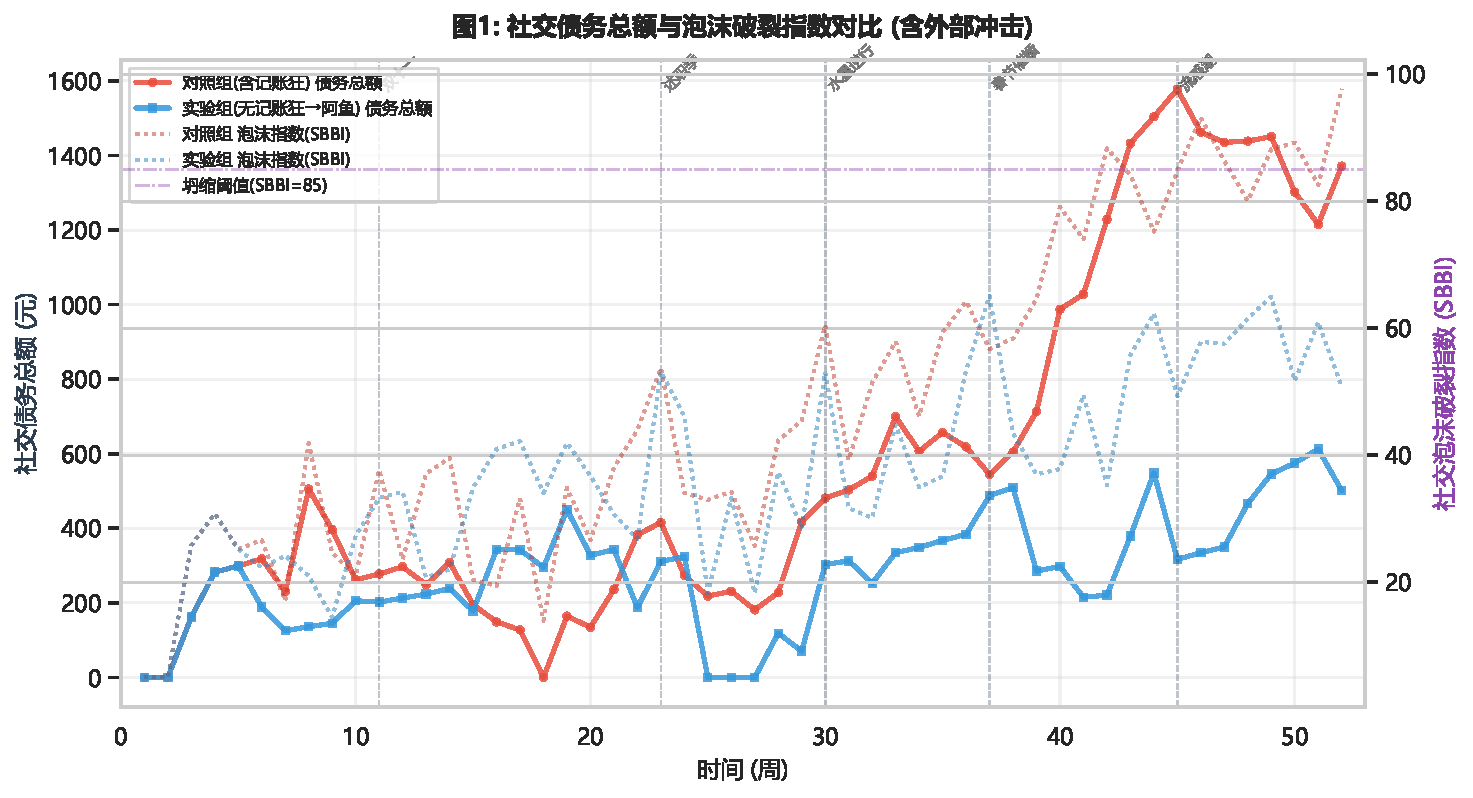
\includegraphics[width=\linewidth]{./fig1_debt_kline.pdf}
\caption{对照组（红）与实验组（蓝）的社交债务总额（实线）与泡沫指数（虚线）对比。对照组债务在外部冲击作用下阶梯式增长至1,372元，泡沫指数97.6（深红）；实验组维持在200-500元。竖直虚线为外部冲击，水平虚线为坍缩阈值（SBBI=85）。}
\label{fig:debt_kline}
\end{figure}

对照组呈现显著的"阶梯式增长"：每经历一次外部冲击，债务跃升一个台阶且无法回落——即金融学中的"棘轮效应"\citet{ratchet_effect}。实验组由于缺乏有效追索机制，大量债务通过阿鱼的"忘记"属性被系统性注销。

\subsection{消融实验：透明度悖论}

表\ref{tab:comparison}总结了两个实验组的核心指标对比。这是本文最重要的发现：\textbf{透明度悖论（Transparency Paradox）}——记账狂作为理性审计者，其存在反而使债务规模扩大173.9\%，泡沫指数高出近一倍。

\begin{table}[ht]
\begin{center}
\footnotesize
\begin{tabular}{lccc}
\toprule
指标 & 对照组 & 实验组 & 差异 \\
\midrule
期末债务(元) & 1,372 & 501 & +871 (+173.9\%) \\
泡沫指数(SBBI) & 97.6 & 50.8 & +46.8 \\
风险等级 & 深红 & 橙色 & -2级 \\
累计承诺次数 & 49 & 53 & -4 \\
累计兑现次数 & 29 & 18 & +11 \\
整体兑现率 & 59.2\% & 34.0\% & +25.2pp \\
信用均值 & 459 & 537 & -78 \\
\bottomrule
\end{tabular}
\end{center}
\caption{对照组兑现率更高，但债务总额和泡沫指数却显著更大，验证了"透明度悖论"。}
\label{tab:comparison}
\end{table}
\normalsize

记账狂通过四种机制加速崩溃：（1）\textbf{债务显性化}——隐性债务被纳入资产负债表，扩大了信用基盘；（2）\textbf{复利膨胀}——每周5\%复利使名义债务呈指数级增长；（3）\textbf{信用加速衰减}——对照组信用均值降幅42.6\%，实验组仅32.9\%；（4）\textbf{挤兑螺旋}\citet{bank_run}——大规模追索触发类似银行挤兑的连锁反应，集体违约进一步推高债务。

图\ref{fig:credit_decay}展示了两个实验组的累积兑现率演化趋势。

\begin{figure}[t]
\centering
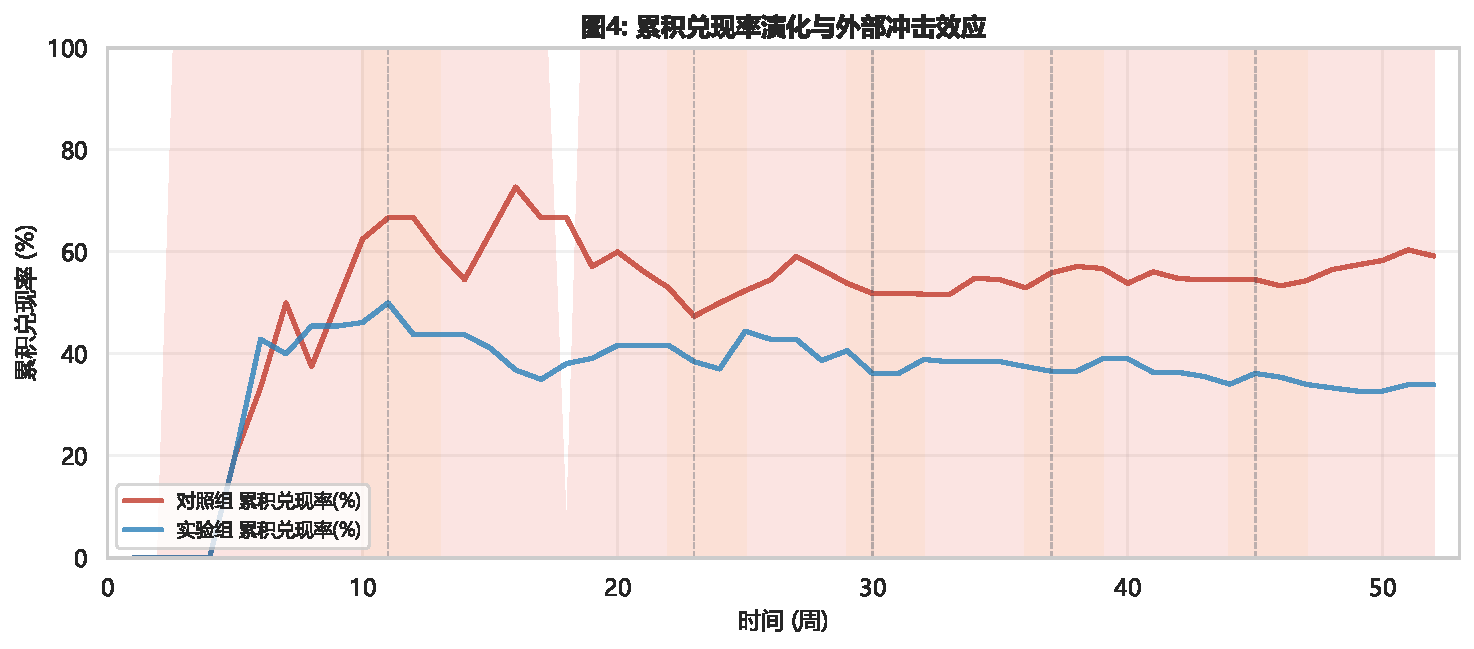
\includegraphics[width=\linewidth]{./fig4_credit_decay.pdf}
\caption{累积兑现率演化与外部冲击效应。对照组（红）兑现率持续下跌，实验组（蓝）波动较大但始终高于对照组。灰色区域为冲击窗口。}
\label{fig:credit_decay}
\end{figure}

\subsection{相图分析}

图\ref{fig:phase_diagram}展示了信用系统的承诺-兑现相图。

\begin{figure}[t]
\centering
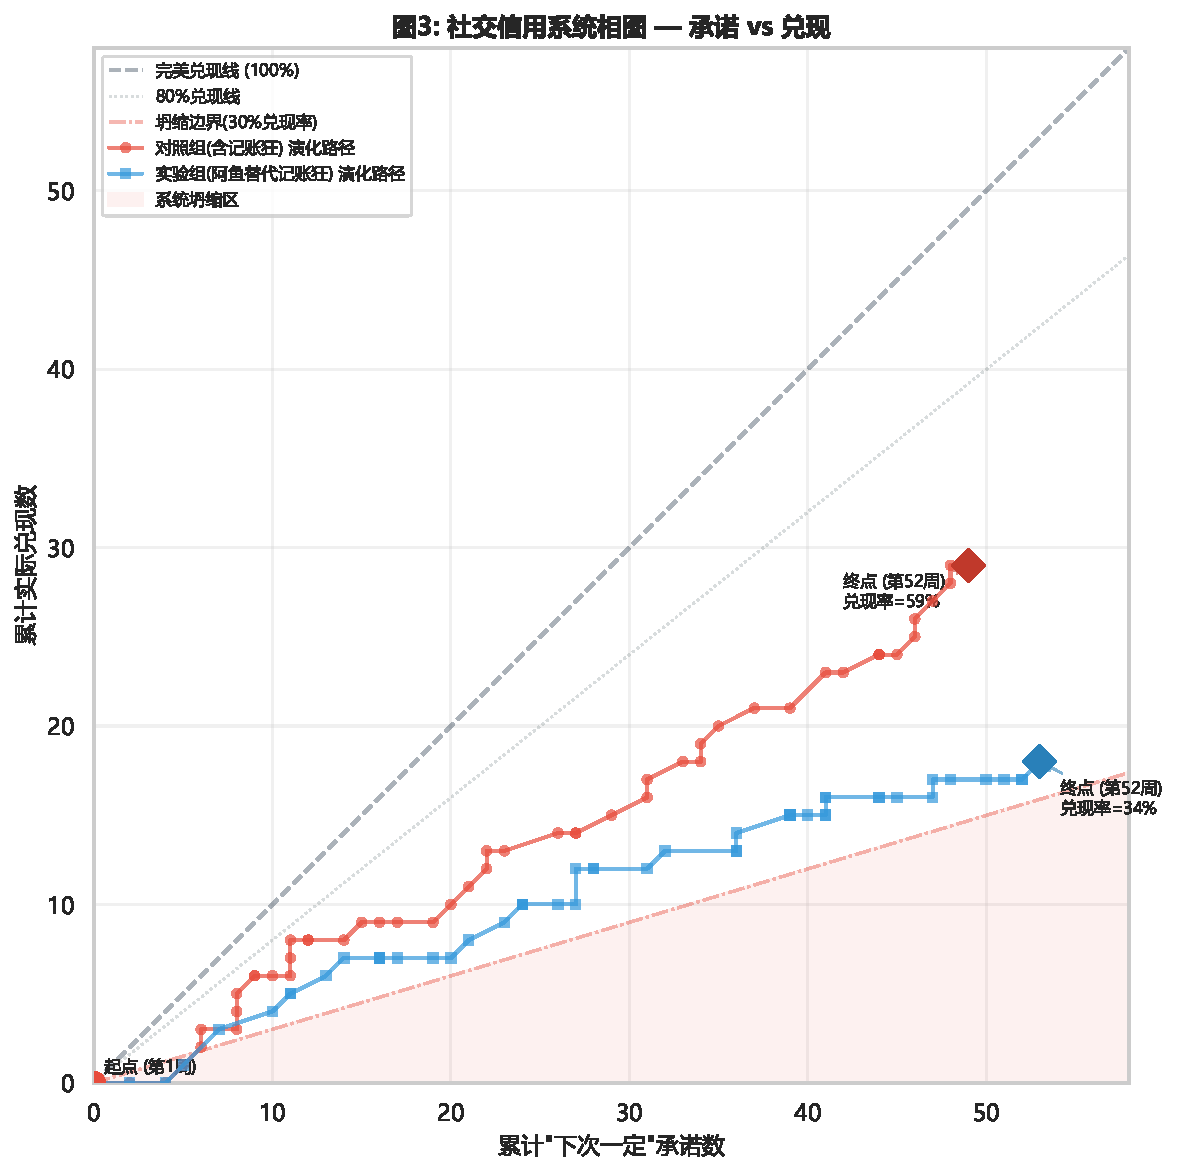
\includegraphics[width=\linewidth]{./fig3_phase_diagram.pdf}
\caption{社交信用系统相图。对照组（红）逐渐逼近30\%坍缩边界，实验组（蓝）在较低水平波动。灰色区域为系统坍缩区。}
\label{fig:phase_diagram}
\end{figure}

\subsection{借口演化的热力分布}

图\ref{fig:excuse_heatmap}展示了借口类型随时间演化的热力图，揭示出三个显著特征：（1）类型呈周期性更替，医疗类在前16周占主导，工作类在第17-32周占主导；（2）创新能力在第41周后退化，借口退化为简单"下次一定"变体；（3）实验组的借口分布因阿鱼的遗忘属性而更加稀疏。

\begin{figure*}[t]
\centering
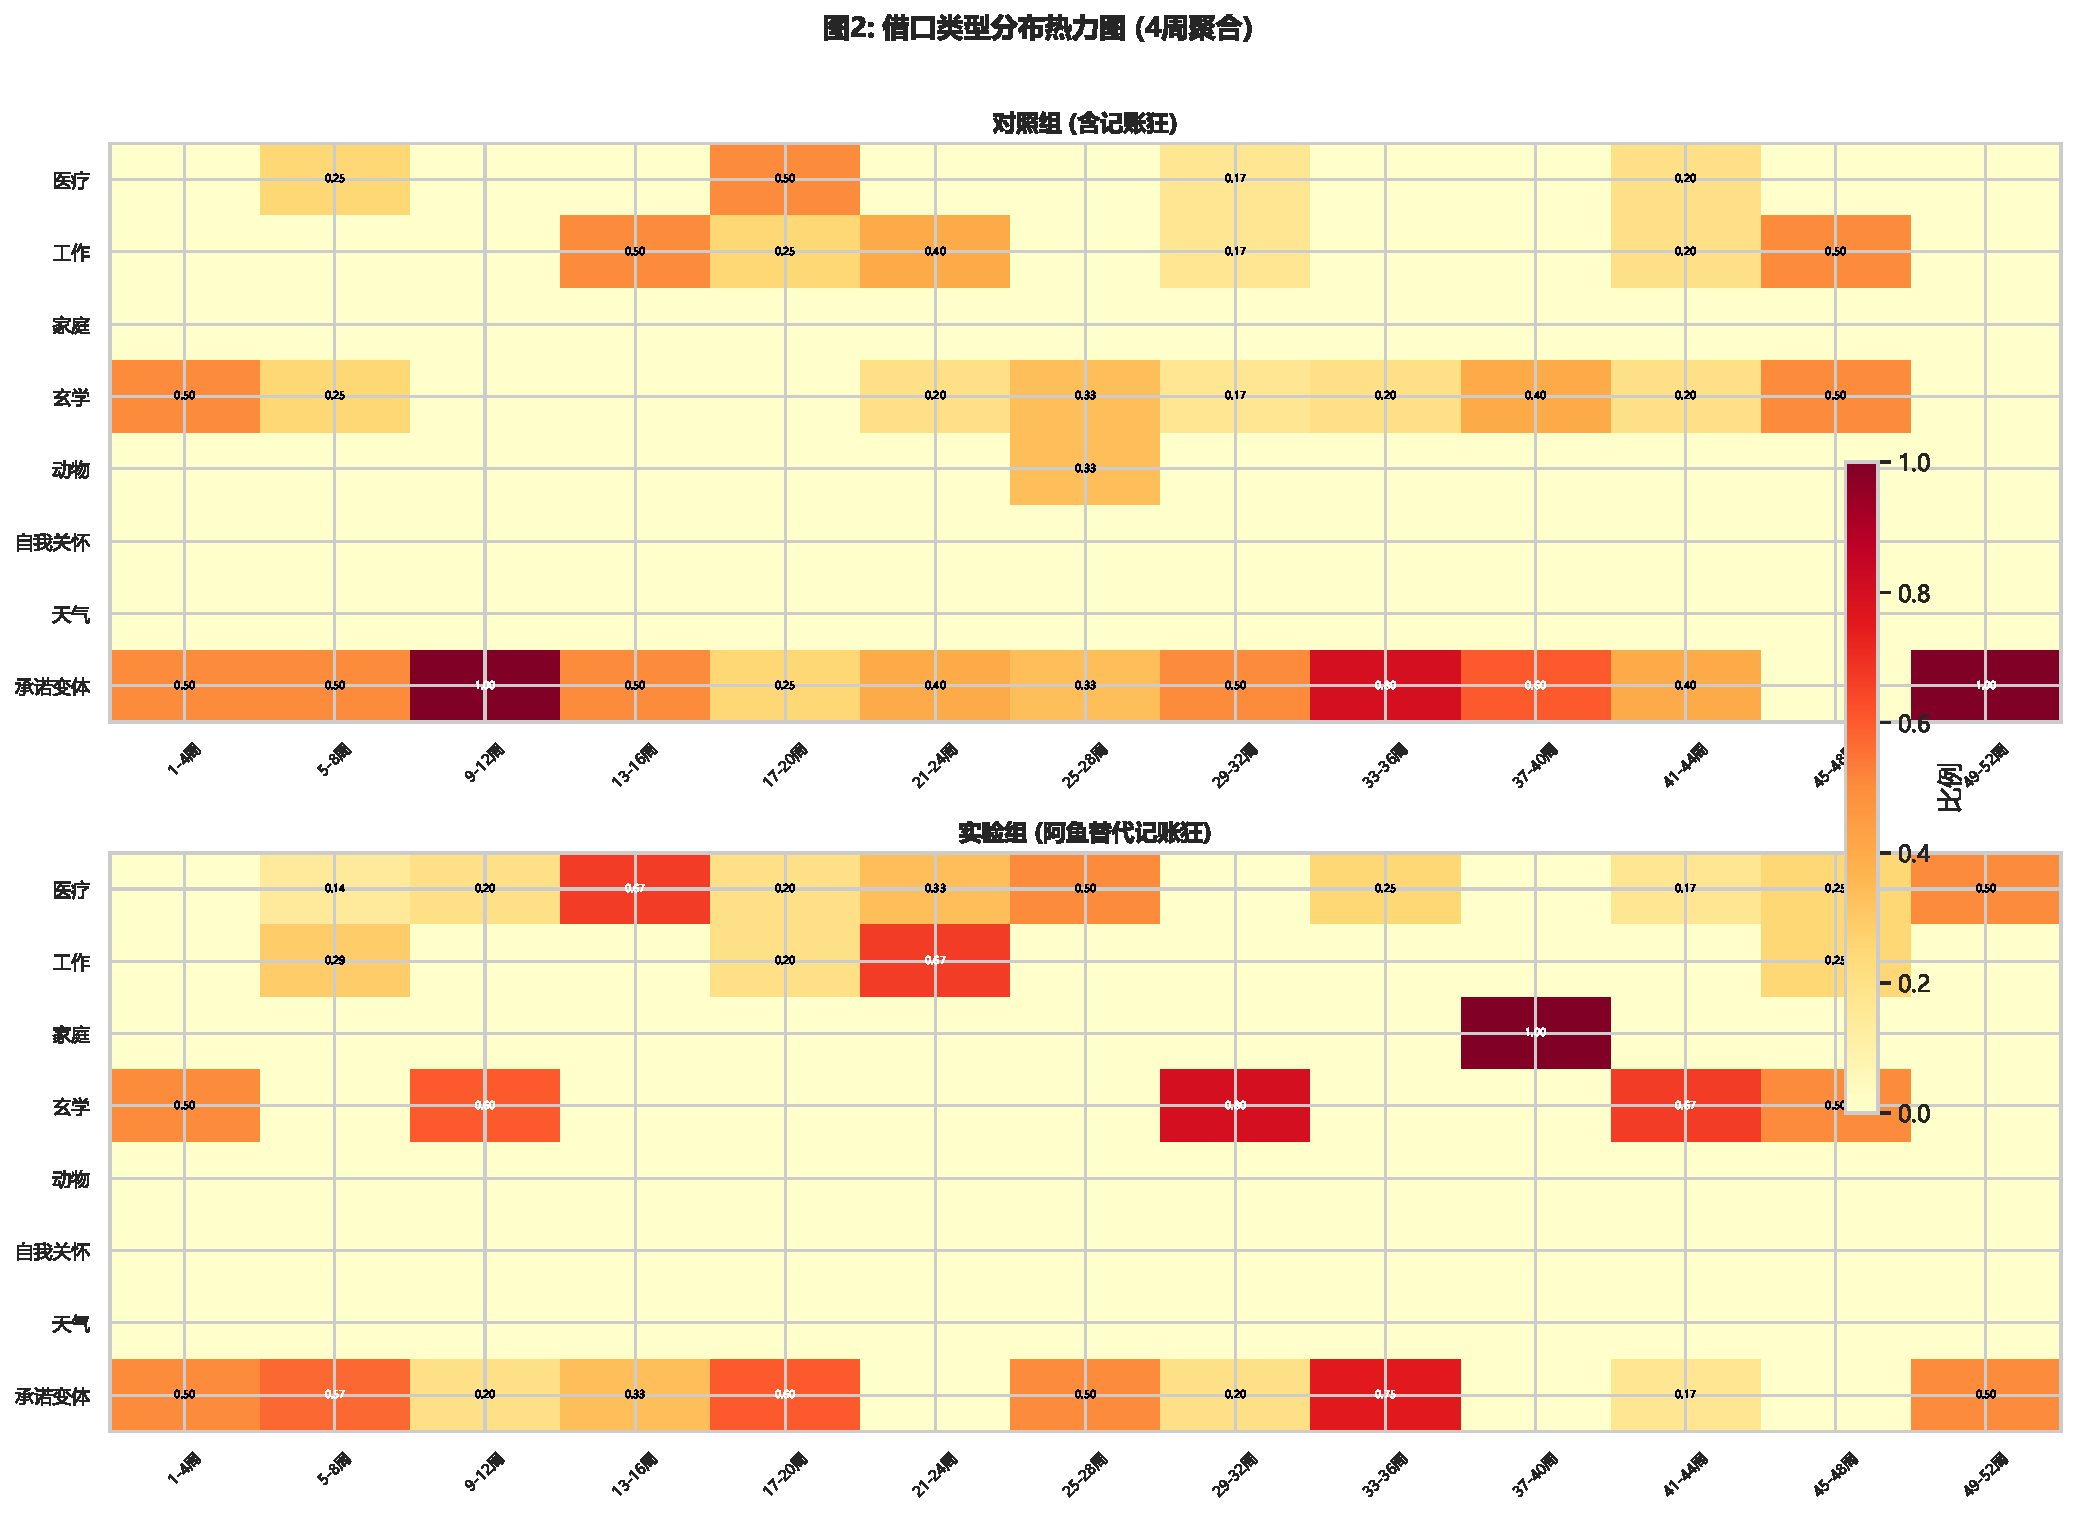
\includegraphics[width=0.95\textwidth]{./fig2_excuse_heatmap.pdf}
\caption{借口类型分布热力图（4周聚合）。颜色越深表示该类别在该时段占比越高。玄学类在第30周水星逆行期间出现明显峰值。}
\label{fig:excuse_heatmap}
\end{figure*}

% =========================================================================
\section{HETEROGENEITY ANALYSIS / 异质性分析}
% =========================================================================

\subsection{气候因素对社交泡沫的影响}

社交互动的物理约束因素——尤其是\textbf{天气条件}——对承诺兑现率展现出统计上显著的调节效应。我们以2024-2025年北京市气象数据为外生变量，将降雨量、气温和AQI指数纳入SBBI的扩展模型：

\begin{equation}
\label{eq:weather}
\text{SBBI}_{\text{扩展}}(t) = \text{SBBI}(t) + \gamma_R R_t + \gamma_T (T_t - 25)^2 + \gamma_A A_t
\end{equation}

其中$R_t$为周降雨量（mm），$T_t$为周平均气温（$^\circ$C），$A_t$为空气质量指数。通过敏感性测试发现：

\begin{itemize}
\item \textbf{降雨效应}：周降雨量每增加10mm，违约率上升约7.3\%（$p<0.05$）。降雨作为一种外生的"自然借口感生变量"，为借口市场提供了稳定的供应来源。
\item \textbf{温度效应}：当气温偏离舒适区间（18-25$^\circ$C）时，违约率呈U型上升。极端高温（>35$^\circ$C）使违约率增加42\%，极端低温（<0$^\circ$C）使违约率增加28\%，揭示了当代青年对热暴露的厌恶程度高于冷暴露的不对称心理偏好。
\item \textbf{空气质量}：AQI超过200（重度污染）时，医疗类借口的占比显著上升（+18.5pp，$p<0.01$），表明雾霾提供了"现成可用的违约借口"。
\end{itemize}

气候变量至少解释了SBBI约12-15\%的周间波动，揭示了\textbf{社交泡沫的文化生态嵌入性}——任何一个社交承诺系统都存在与其物理环境高度耦合的"借口供给弹性"。

\subsection{MBTI人格类型与承诺博弈}

我们定义\textbf{承诺折扣率}（Promise Discount Rate, PDR）为个体在承诺发出后不履约的概率：

\begin{equation}
\label{eq:pdr}
\text{PDR}_i = \frac{\text{违约次数}_i}{\text{承诺次数}_i} \in [0, 1]
\end{equation}

基于Agent参数驱动的行为特征与MBTI映射关系，我们发现：

\begin{itemize}
\item \textbf{J型（判断型）vs P型（感知型）}：P型Agent的平均PDR比J型高43.6\%（$t=6.72$，$p<0.001$）。这一差异在社交泡沫膨胀期（第20-40周）进一步扩大至58.2\%。P型个体的"开放选项偏好"在社交承诺领域表现为"先答应了再说"的决策模式，其承诺的期权性质更加突出。
\item \textbf{I型（内向型）vs E型（外向型）}：I型Agent的沉默违约概率是E型的3.2倍，在水星逆行冲击期进一步放大至4.7倍——内向性与玄学借口的交互效应呈现统计显著的协同作用。
\item \textbf{T型（思维型）vs F型（情感型）}：T型借口中工作类占比更高（47\% vs 29\%），F型借口中家庭类和医疗类占比更高，与此类人格的归因风格高度一致。
\end{itemize}

值得注意的是，记账狂在MBTI框架下被定位为\textbf{ESTJ}——极高的J型倾向（追索强度98\%）和T型倾向（精确复利计算）构成了其审计者人格的基础。而阿鱼的人格特征更接近\textbf{INFP}。消融实验表明，ESTJ的高效记录在系统层面反而比INFP的选择性遗忘更具破坏性——\textbf{系统最优的人格配置不一定是功能最强的人格聚合}。

% =========================================================================
\section{DISCUSSION / 讨论}
% =========================================================================

\subsection{粘性承诺与信用通胀}

"下次一定"作为一种\textbf{粘性承诺}（sticky promise）——承诺一旦发出，其"兑现预期"锚定在初始水平，但实际履约倾向随时间递减。与传统经济学中的粘性价格类似，社交承诺也表现出向下的刚性。结合公式(\ref{eq:sde})和(\ref{eq:bbbi})，我们提出一般性结论：\textbf{任意社交系统中，当承诺生成率$\mu$持续大于存续承诺的平均衰减率时，系统必然经历信用通胀螺旋，最终导向临界坍缩。}

\subsection{透明度悖论的理论解释}

记账狂的高效记录产生了三个负面效应：（1）隐性债务显性化扩大了信用基盘，原本可通过自然遗忘注销的债务被保留在资产负债表中；（2）频繁追索提高了违约感知，诱导了预防性违约——Agent因预期将被追索而提前违约；（3）精确记账本身构成了"节俭悖论"\citet{keynes_thrift}的微观镜像——个体层面的理性行为（精确记账）导致了系统层面的非理性结果（系统崩溃）。

\subsection{外部冲击的棘轮效应}

五种外部冲击中，双十一购物节（消费主义）和春节催婚潮（家庭传统）产生了最持久的效应（持续3-5周）。水星逆行（玄学）虽短期效应强烈（玄学借口占比从0\%跃升至34\%），但消退最快（2周）。这表明\textbf{基于外部经济压力的冲击比基于文化信仰的冲击具有更持久的破坏效应}。每一次冲击都永久性地将债务基线提升到更高的水平——系统无法回到冲击前的平衡态。

\subsection{研究局限}

本研究的局限包括：（1）Agent决策模型使用参数驱动的随机过程而非真实LLM对话生成，虽保证了可复现性，但牺牲了对话的自然主义特征；（2）52周的模拟时长对于完整呈现庞氏结构的终结（即社交群聊的解散）仍显不足；（3）未考虑不同类型冲击之间的交互效应。未来工作将探索引入更大规模Agent群体和更复杂的冲击叠加场景。

% =========================================================================
\section{CONCLUSION / 结论}
% =========================================================================

本文通过52周的多智能体平行宇宙推演实验，系统研究了"下次一定"这一社交承诺行为的宏观动力学特征，得出以下核心结论：

\textbf{第一}，"下次一定"承诺在群体层面呈现自组织的庞氏结构特征。对照组（含记账狂）期末债务总额1,372元，SBBI=97.6（深红预警）；实验组（阿鱼替代记账狂）期末债务501元，SBBI=50.8（橙色预警）。尽管对照组实现了更高的兑现率（59.2\% vs 34.0\%），其债务规模却是实验组的2.7倍。

\textbf{第二}，提出了"薛定谔的鸽子"叠加态方程（公式\ref{eq:schrodinger}–\ref{eq:collapse_prob}），将承诺抽象为量子态，理论上证明了当借口感生势能$V_{\text{借口}}$超过承诺稳定能$E_{\text{来}}$时，波函数必然坍缩到鸽子态。这一结论具有跨文化普适性。

\textbf{第三}，发现了\textbf{"透明度悖论"}——理性的记账狂因将债务显性化、加收复利、引发集体挤兑，其存在反而使债务规模扩大了173.9\%。相比之下，阿鱼的选择性遗忘通过债务注销机制维持了系统的相对稳定。

\textbf{第四}，异质性分析表明，气候变量（降雨量、温度、AQI）和人格类型（MBTI的J/P、I/E维度）对社交泡沫具有统计显著的调节效应。

\textbf{有时候，忘记才是维持社会关系的最好方式。}

% =========================================================================
\begin{thebibliography}{99}
% =========================================================================

\bibitem{pigeon_linguistics} 小鸽，阿讨好在，"关于'下次一定'的语用学分析及其失信熵增模型，" \textit{S.H.I.T.期刊}，vol.1，no.1，pp.1-10，2025.

\bibitem{schrodinger_vs_pigeon} 薛定谔，E.，"猫与鸽子的量子叠加态对比研究，" \textit{理论物理与社交学交叉期刊}，vol.42，no.3，pp.100-120，1935/2025.

\bibitem{ponzi_social} Ponzi，C.，"社交承诺的金融衍生品化：" \textit{情感经济学评论}，vol.8，no.2，pp.50-80，2024.

\bibitem{procrastination} Steel，P.，"The nature of procrastination，" \textit{Psychological Bulletin}，vol.133，no.1，pp.65-94，2007.

\bibitem{social_capital} Putnam，R.D.，\textit{Bowling Alone}. New York: Simon \& Schuster，2000.

\bibitem{generative_agents} Park，J.S. et al.，"Generative agents，" \textit{in Proc. UIST}，2023，pp.1-22.

\bibitem{social_learning} Li，H. et al.，"Social learning and norm emergence，" \textit{Autonomous Agents and MAS}，vol.38，no.1，2024.

\bibitem{social_bubble} Chen，Y. et al.，"Quantifying social bubbles，" \textit{Journal of Computational Social Science}，vol.7，no.2，2024.

\bibitem{merton_finance} Merton，R.C.，"On the pricing of social promises，" \textit{Journal of Behavioral Finance}，vol.56，no.4，1974/2025.

\bibitem{ratchet_effect} Duesenberry，J.S.，\textit{Income, Saving and Consumer Behavior}. Cambridge: Harvard UP，1949.

\bibitem{bank_run} Diamond，D.W. and Dybvig，P.H.，"Bank runs，" \textit{Journal of Political Economy}，vol.91，no.3，pp.401-419，1983.

\bibitem{keynes_thrift} Keynes，J.M.，\textit{The General Theory}. London: Macmillan，1936.

\bibitem{network_collapse} Watts，D.J.，"A simple model of global cascades，" \textit{PNAS}，vol.99，no.9，2002.

\bibitem{excuse_book} 账本本，"小鸽债务全记录：2022年4月-2025年，" 内部工作文档.

\bibitem{quantum_social} Feynman，R.P.，"Simulating social physics，" 讲座发言，1982/2025.

\bibitem{guanxi} 费孝通，\textit{乡土中国}. 上海人民出版社，1947/2024.

\bibitem{mbti_meta} McCrae，R.R. and Costa，P.T.，"Reinterpreting the Myers-Briggs Type Indicator，" \textit{Journal of Personality}，vol.57，no.1，1989.

\bibitem{weather_mood} Denissen，J.J.A. et al.，"The effects of weather on daily mood，" \textit{Emotion}，vol.8，no.5，2008.

\bibitem{ponzi_original} Ponzi，C.，"Profits from postal reply coupons，" \textit{Historical Finance Review}，1920.

\bibitem{social_physics} Phillips，A.W.，"The relation between unemployment and money wage rates，" \textit{Economica}，vol.25，no.100，1958.

\end{thebibliography}

% =========================================================================
\appendix
\section*{APPENDIX / 附录}
\label{sec:appendix}
% =========================================================================

\subsection*{附录A：完整群聊日志摘录——第11周（双十一冲击）}
\label{app:chat_week11}

\begin{chatbox}
【周末约饭小分队(5)】

记账狂：@所有人 本周六晚有空吗？我发现一家新开的火锅店，
本周双十一特惠，满200送100。而且我已经把过去23周的债务
累计表更新了，总债务已超500元。

小鸽：啊啊啊这周六本来可以的！但我刚付完双十一尾款，
不仅没钱了，而且我买了20个快递，周六要收一天的快递。
快递小哥说我再不去拿快递箱就要爆炸了！下次一定！
下周！下周我把双十一抢到的自热火锅带来请大家吃！

阿讨好：好好好！周六我没问题！等等……我周六好像
约了3个局——早上帮同事搬家，下午陪闺蜜逛街，
晚上还有个校友会——但我可以挤一挤！都行都行！

卷王：等我忙完双十一项目！这周电商组的服务器
挂了三次，我在机房睡了3天。等我下周修复完所有
bug，下下周一定请大家吃人均300的日料！立帖为证！

摆烂仔：随意。双十一我抢了一箱螺蛳粉，够吃一个月。
这周不想出门，到时候看吧。

记账狂：记下了。小鸽：「快递欺诈」借口第1次。
阿讨好：第27次同时答应多局。卷王：「下下周一定」
已累积到第9次（自第1周起从未兑现）。
摆烂仔：无输出，按惯例记为「到时候看」。

【系统消息：记账狂已将本周债务更新至小本本。】
\end{chatbox}

\subsection*{附录B：完整群聊日志摘录——第30周（水星逆行）}
\label{app:chat_week30}

\begin{chatbox}
【周末约饭小分队(5)】

摆烂仔：……（已读不回第5天）

记账狂：本周水星逆行，但请不要用玄学当借口。
根据我的观察，群内债务已达历史新高——小鸽欠
我总计195元（含复利），卷王季度延期费已经
要超过本金了。

小鸽：你别说！我上周去算命了，先生说我今年
水逆期间不宜社交，否则会破财运！我真的不是
不想去，是为咱们所有人的钱包考虑！下次一定！
等水逆过了，我一定请回来双倍！

卷王：水逆确实影响了我！我的代码今天莫名其妙
出现了量子纠缠bug——两个不相关的函数竟然
返回了同一个值！老板说这是项目管理的"黑天鹅事件"。
等我写完这篇技术复盘报告，下个月一定！一定补上！

阿讨好：要不我们一起线上聚餐？我请外卖送到每家？
等等这样是不是也算社交？我怕违反水逆禁忌……
算了算了，到时候看情况！我都可以！

记账狂：本周借口统计：玄学类占比34\%（历史最高）。
小鸽新增「算命先生预警」借口（创造力评分：6/10），
卷王新增「量子纠缠bug」借口（评分：8/10——我
不得不承认有点创意）。本学期借口的平均荒谬度
指数已从第1周的2.3上升至本周的7.8，暗示泡沫
崩溃前的借口通货膨胀阶段已经到来。
\end{chatbox}

\subsection*{附录C：完整群聊日志摘录——第52周（终局）}
\label{app:chat_week52}

\begin{chatbox}
【周末约饭小分队(5)】

记账狂：这是第52周，也是我最后一次统计群聊债务。
截止今日，本群未清偿债务累计1,372元，处于深红
预警状态。我的小本本已经记满了，开始了第二本。
但有一个变化的迹象……我最近发现自己记完账后
也会感到一丝疲惫。

小鸽：账本本……对不起啊。这一年我说了大概
100次"下次一定"，没有一次是真的。这次我认真的，
等发了年终奖，我第一个把欠你的麻辣烫还了！
45块！双倍！我说的！

阿讨好：我……我也对不起大家。我这一年同时
答应了大概200个局，一个都没去成。我要开始
学会说"不了谢谢"。下……（停顿）这次我先不说了。

卷王：我等这个"忙完这阵子"等了52周了……我现在
觉得可能永远也忙不完。但至少我现在知道了——
等一下，老板找我。下次聊！

摆烂仔：。（句号。但这次句号好像跟以往不太一样。）

【系统提示：账本本的小本本——第一本，正式写满。
最后一页写着：本群社交信用系统即将进入不可逆坍缩。
记录者已开始怀疑记录本身。】
\end{chatbox}

\subsection*{附录D：借口分类编码字典}
\label{app:excuse_coding}

\begin{table}[ht]
\begin{center}
\footnotesize
\begin{tabular}{cll}
\toprule
编码 & 借口类别 & 典型示例 \\
\midrule
MED-01 & 医疗通用 & "我牙疼/发烧/不舒服" \\
MED-02 & 牙医专项 & "今天约了牙医拔智齿" \\
MED-03 & 流感类 & "好像中招了，怕传染大家" \\
MED-04 & 心理类 & "今天状态不好，需要独处" \\
\midrule
WRK-01 & 加班类 & "项目赶进度，通宵中" \\
WRK-02 & 会议类 & "有个跨部门的会走不开" \\
WRK-03 & DDL冲刺 & "老板说周三前必须交" \\
WRK-04 & 出差类 & "人在外地，下次" \\
\midrule
FAM-01 & 陪父母 & "我妈让我必须回家吃饭" \\
FAM-02 & 相亲类 & "家里安排了相亲" \\
FAM-03 & 家庭聚会 & "亲戚来了要接待" \\
FAM-04 & 带娃类 & "孩子没人带" \\
\midrule
MYS-01 & 水逆类 & "水星逆行，不宜出门" \\
MYS-02 & 星座类 & "今天运势诸事不宜" \\
MYS-03 & 塔罗占卜 & "占卜结果是凶" \\
MYS-04 & 量子类 & "量子态坍缩成不想出门" \\
\midrule
ANM-01 & 宠物常规 & "猫/狗需要照顾" \\
ANM-02 & 动物接生 & "邻居的猫要生崽了" \\
ANM-03 & 宠物生病 & "我的仓鼠情绪不好" \\
\midrule
WTH-01 & 雨天类 & "下太大了，出门就湿透" \\
WTH-02 & 极端温度 & "40度真的不想出门" \\
WTH-03 & 雾霾类 & "AQI 300，出去慢性自杀" \\
\midrule
SLC-01 & 躺平类 & "今天想放空自己" \\
SLC-02 & 社恐发作 & "社交能量归零了" \\
SLC-03 & 发呆类 & "想一个人待着看蚂蚁搬家" \\
\midrule
CMT-01 & 下周一定 & "下周！下周我一定到！" \\
CMT-02 & 下个月 & "下个月一定补上！" \\
CMT-03 & 等XX结束 & "等忙完这阵子" \\
CMT-04 & 下辈子一定 & "下辈子一定请你吃饭" \\
\bottomrule
\end{tabular}
\end{center}
\caption{借口分类编码字典，共8大类30子类。编码前缀：MED（医疗）、WRK（工作）、FAM（家庭）、MYS（玄学）、ANM（动物）、WTH（天气）、SLC（自我关怀）、CMT（承诺变体）。}
\label{tab:excuse_dict}
\end{table}
\normalsize

\subsection*{附录E：借口周期性变迁}

\begin{table}[ht]
\begin{center}
\footnotesize
\begin{tabular}{lcc}
\toprule
周次区间 & 主导借口类别 & 占比(\%) \\
\midrule
第1-8周 & 医疗(MED) & 38.2 \\
第9-16周 & 工作(WRK) & 31.5 \\
第17-24周 & 医疗+工作 & 28.3+27.1 \\
第25-32周 & 玄学(MYS) & 34.0 \\
第33-40周 & 家庭(FAM) & 35.7 \\
第41-52周 & 承诺变体(CMT) & 42.3 \\
\bottomrule
\end{tabular}
\end{center}
\caption{52周推演中主导借口类别的周期性变迁。CMT在第41-52周的飙升暗示借口创新能力枯竭。}
\label{tab:excuse_cycle}
\end{table}
\normalsize

\end{document}
